%!TEX TS-program = xelatex
\documentclass[11pt]{article}

\usepackage[english]{babel}

\usepackage{amsmath,amssymb,amsfonts}
\usepackage[utf8]{inputenc}
\usepackage[T1]{fontenc}
\usepackage{stix2}
\usepackage[scaled]{helvet}
\usepackage[scaled]{inconsolata}

\usepackage{lastpage}

\usepackage{setspace}

\usepackage{ccicons}

\usepackage[hang,flushmargin]{footmisc}

\usepackage{geometry}

\setlength{\parindent}{0pt}
\setlength{\parskip}{6pt plus 2pt minus 1pt}

\usepackage{fancyhdr}
\renewcommand{\headrulewidth}{0pt}\providecommand{\tightlist}{%
  \setlength{\itemsep}{0pt}\setlength{\parskip}{0pt}}

\makeatletter
\newcounter{tableno}
\newenvironment{tablenos:no-prefix-table-caption}{
  \caption@ifcompatibility{}{
    \let\oldthetable\thetable
    \let\oldtheHtable\theHtable
    \renewcommand{\thetable}{tableno:\thetableno}
    \renewcommand{\theHtable}{tableno:\thetableno}
    \stepcounter{tableno}
    \captionsetup{labelformat=empty}
  }
}{
  \caption@ifcompatibility{}{
    \captionsetup{labelformat=default}
    \let\thetable\oldthetable
    \let\theHtable\oldtheHtable
    \addtocounter{table}{-1}
  }
}
\makeatother

\usepackage{array}
\newcommand{\PreserveBackslash}[1]{\let\temp=\\#1\let\\=\temp}
\let\PBS=\PreserveBackslash

\usepackage[breaklinks=true]{hyperref}
\hypersetup{colorlinks,%
citecolor=blue,%
filecolor=blue,%
linkcolor=blue,%
urlcolor=blue}
\usepackage{url}

\usepackage{caption}
\setcounter{secnumdepth}{0}
\usepackage{cleveref}

\usepackage{graphicx}
\makeatletter
\def\maxwidth{\ifdim\Gin@nat@width>\linewidth\linewidth
\else\Gin@nat@width\fi}
\makeatother
\let\Oldincludegraphics\includegraphics
\renewcommand{\includegraphics}[1]{\Oldincludegraphics[width=\maxwidth]{#1}}

\usepackage{longtable}
\usepackage{booktabs}

\usepackage{color}
\usepackage{fancyvrb}
\newcommand{\VerbBar}{|}
\newcommand{\VERB}{\Verb[commandchars=\\\{\}]}
\DefineVerbatimEnvironment{Highlighting}{Verbatim}{commandchars=\\\{\}}
% Add ',fontsize=\small' for more characters per line
\usepackage{framed}
\definecolor{shadecolor}{RGB}{248,248,248}
\newenvironment{Shaded}{\begin{snugshade}}{\end{snugshade}}
\newcommand{\KeywordTok}[1]{\textcolor[rgb]{0.13,0.29,0.53}{\textbf{#1}}}
\newcommand{\DataTypeTok}[1]{\textcolor[rgb]{0.13,0.29,0.53}{#1}}
\newcommand{\DecValTok}[1]{\textcolor[rgb]{0.00,0.00,0.81}{#1}}
\newcommand{\BaseNTok}[1]{\textcolor[rgb]{0.00,0.00,0.81}{#1}}
\newcommand{\FloatTok}[1]{\textcolor[rgb]{0.00,0.00,0.81}{#1}}
\newcommand{\ConstantTok}[1]{\textcolor[rgb]{0.00,0.00,0.00}{#1}}
\newcommand{\CharTok}[1]{\textcolor[rgb]{0.31,0.60,0.02}{#1}}
\newcommand{\SpecialCharTok}[1]{\textcolor[rgb]{0.00,0.00,0.00}{#1}}
\newcommand{\StringTok}[1]{\textcolor[rgb]{0.31,0.60,0.02}{#1}}
\newcommand{\VerbatimStringTok}[1]{\textcolor[rgb]{0.31,0.60,0.02}{#1}}
\newcommand{\SpecialStringTok}[1]{\textcolor[rgb]{0.31,0.60,0.02}{#1}}
\newcommand{\ImportTok}[1]{#1}
\newcommand{\CommentTok}[1]{\textcolor[rgb]{0.56,0.35,0.01}{\textit{#1}}}
\newcommand{\DocumentationTok}[1]{\textcolor[rgb]{0.56,0.35,0.01}{\textbf{\textit{#1}}}}
\newcommand{\AnnotationTok}[1]{\textcolor[rgb]{0.56,0.35,0.01}{\textbf{\textit{#1}}}}
\newcommand{\CommentVarTok}[1]{\textcolor[rgb]{0.56,0.35,0.01}{\textbf{\textit{#1}}}}
\newcommand{\OtherTok}[1]{\textcolor[rgb]{0.56,0.35,0.01}{#1}}
\newcommand{\FunctionTok}[1]{\textcolor[rgb]{0.00,0.00,0.00}{#1}}
\newcommand{\VariableTok}[1]{\textcolor[rgb]{0.00,0.00,0.00}{#1}}
\newcommand{\ControlFlowTok}[1]{\textcolor[rgb]{0.13,0.29,0.53}{\textbf{#1}}}
\newcommand{\OperatorTok}[1]{\textcolor[rgb]{0.81,0.36,0.00}{\textbf{#1}}}
\newcommand{\BuiltInTok}[1]{#1}
\newcommand{\ExtensionTok}[1]{#1}
\newcommand{\PreprocessorTok}[1]{\textcolor[rgb]{0.56,0.35,0.01}{\textit{#1}}}
\newcommand{\AttributeTok}[1]{\textcolor[rgb]{0.77,0.63,0.00}{#1}}
\newcommand{\RegionMarkerTok}[1]{#1}
\newcommand{\InformationTok}[1]{\textcolor[rgb]{0.56,0.35,0.01}{\textbf{\textit{#1}}}}
\newcommand{\WarningTok}[1]{\textcolor[rgb]{0.56,0.35,0.01}{\textbf{\textit{#1}}}}
\newcommand{\AlertTok}[1]{\textcolor[rgb]{0.94,0.16,0.16}{#1}}
\newcommand{\ErrorTok}[1]{\textcolor[rgb]{0.64,0.00,0.00}{\textbf{#1}}}
\newcommand{\NormalTok}[1]{#1}

\newlength{\cslhangindent}
\setlength{\cslhangindent}{1.5em}
\newlength{\csllabelwidth}
\setlength{\csllabelwidth}{3em}
\newenvironment{CSLReferences}[3] % #1 hanging-ident, #2 entry spacing
 {% don't indent paragraphs
  \setlength{\parindent}{0pt}
  % turn on hanging indent if param 1 is 1
  \ifodd #1 \everypar{\setlength{\hangindent}{\cslhangindent}}\ignorespaces\fi
  % set entry spacing
  \ifnum #2 > 0
  \setlength{\parskip}{#2\baselineskip}
  \fi
 }%
 {}
\usepackage{calc} % for \widthof, \maxof
\newcommand{\CSLBlock}[1]{#1\hfill\break}
\newcommand{\CSLLeftMargin}[1]{\parbox[t]{\maxof{\widthof{#1}}{\csllabelwidth}}{#1}}
\newcommand{\CSLRightInline}[1]{\parbox[t]{\linewidth}{#1}}
\newcommand{\CSLIndent}[1]{\hspace{\cslhangindent}#1}\geometry{verbose,letterpaper,tmargin=2.2cm,bmargin=2.2cm,lmargin=2.2cm,rmargin=2.2cm}

\usepackage{lineno}
\usepackage[nolists,noheads]{endfloat}

\pagestyle{plain}

\tolerance=1
\emergencystretch=\maxdimen
\hyphenpenalty=10000
\hbadness=10000

\doublespacing

\fancypagestyle{normal}
{
  \fancyhf{}
  \fancyfoot[R]{\footnotesize\sffamily\thepage\ of \pageref*{LastPage}}
}
\begin{document}
\raggedright
\thispagestyle{empty}
{\Large\bfseries\sffamily NeutralLandscapes.jl: a library for efficient
generation of neutral landscapes with temporal change}
\vskip 5em

%
\href{https://orcid.org/0000-0002-6506-6487}{Michael D.\,Catchen}%
%
\,\textsuperscript{1,2}

\textsuperscript{1}\,McGill University\quad \textsuperscript{2}\,Québec
Centre for Biodiversity Sciences


\textbf{Correspondance to:}\\
Michael D. Catchen --- \texttt{michael.catchen@mail.mcgill.ca}\\

\vfill
This work is released by its authors under a CC-BY 4.0 license\hfill\ccby\\
Last revision: \emph{\today}

\clearpage
\thispagestyle{empty}

\vfill
Soon to be a paper, maybe. TK authors, MKB,VB,RS,TP



\vfill

\clearpage
\linenumbers
\pagestyle{normal}

\hypertarget{introduction}{%
\section{Introduction}\label{introduction}}

\begin{itemize}
\tightlist
\item
  what are neutral landscapes
\end{itemize}

Neutral landscapes are increasingly used in ecological and evolutionary
studies to provide a null expectation spatial variation of some
measurement.

Different properties of landscapes (elevation, land cover, temperature)
vary across space in non-random ways. Tobler's law of geography:
``everything is related to everything else, but near things are more
related than distant things''

Originally based around methods for simulating spatially auto-correlated
data (Gardner \emph{et al.} 1987; Milne 1992).

they have seen use in a wide range of fields in ecology and evolution:
from landscape genetics (Storfer \emph{et al.} 2007), to spatial ecology
(Tinker \emph{et al.} 2004; Remmel \& Fortin 2013), and biogeography
(Albert \emph{et al.} 2017).

The two most popular libraries used to generate neutral landscapes are
\texttt{NLMR} in (the \texttt{R} language) (Sciaini \emph{et al.} 2018)
and \texttt{NLMpy} (in Python; Etherington \emph{et al.} 2015). Here we
present \texttt{NeutralLandscapes.jl}, a new package for neutral
landscape simulation in the \texttt{Julia} language. So, why create
another package?

Here we demonstrate that \texttt{NeutralLandscapes.jl} is orders of
magnitude faster than previous neutral landscape packages.

In addition, \texttt{NeutralLandscapes.jl} implements several novel
methods for simulating environmental change with temporal variation. As
biodiversity science becomes increasingly concerned with temporal change
and its consequences, its clear there is a gap in methodology in
generating neutral landscapes that change over time. Our model allows
users to simulate time-series of any \texttt{NeutralLandscape} layer,
and which can produce an arbitrary distribution of change across every
spatial cell, with provided levels of spatial and temporal
autocorrelation.

\hypertarget{software-overview}{%
\section{Software Overview}\label{software-overview}}

This software can generate neutral landscapes using several methods,
enables masking and works with other julia packages.

fig.~\ref{fig:allmethods} shows a replica of Figure 1 from Etherington
\emph{et al.} (2015), which shows the capacity of the library to
generate different types of neutral landscapes, and then apply masks and
categorical classifcation to them.

\begin{figure}
\hypertarget{fig:allmethods}{%
\centering
\includegraphics{./figures/figure1.png}
\caption{Recreation of the figure in \texttt{nlmpy} paper and the
source, supplied in less than 40 lines of code.}\label{fig:allmethods}
}
\end{figure}

Further, \texttt{NL.jl} provides methods for interacting with other
\texttt{julia} packages, and functions for rescaling

\hypertarget{interoperability}{%
\subsection{Interoperability}\label{interoperability}}

Ease of use with other julia packages

Mask of neutral variable masked across quebec in 3 lines.

\begin{verbatim}
using NeutralLandscapes
using SimpleSDMLayers

quebec = SimpleSDMPredictor(WorldClim, BioClim; left=-90., right=-50., top=75., bottom=40.)
qcmask = fill(true, size(quebec))                   # ------ TODO
qcmask[findall(isnothing, quebec.grid)] .= false    # should both of these lines be possible only using mask?

pltsettings = (cbar=:none, frame=:box)

plot(
    heatmap(rand(MidpointDisplacement(0.8), size(layer), mask=qcmask); pltsettings),
    heatmap(rand(PlanarGradient(), size(layer), mask=qcmask); pltsettings),
    heatmap(rand(PerlinNoise((4,4)), size(layer), mask=qcmask); pltsettings),
    heatmap(rand(NearestNeighborCluster(0.5), size(layer), mask=qcmask); pltsettings),
    dpi=400
)
\end{verbatim}

\begin{figure}
\centering
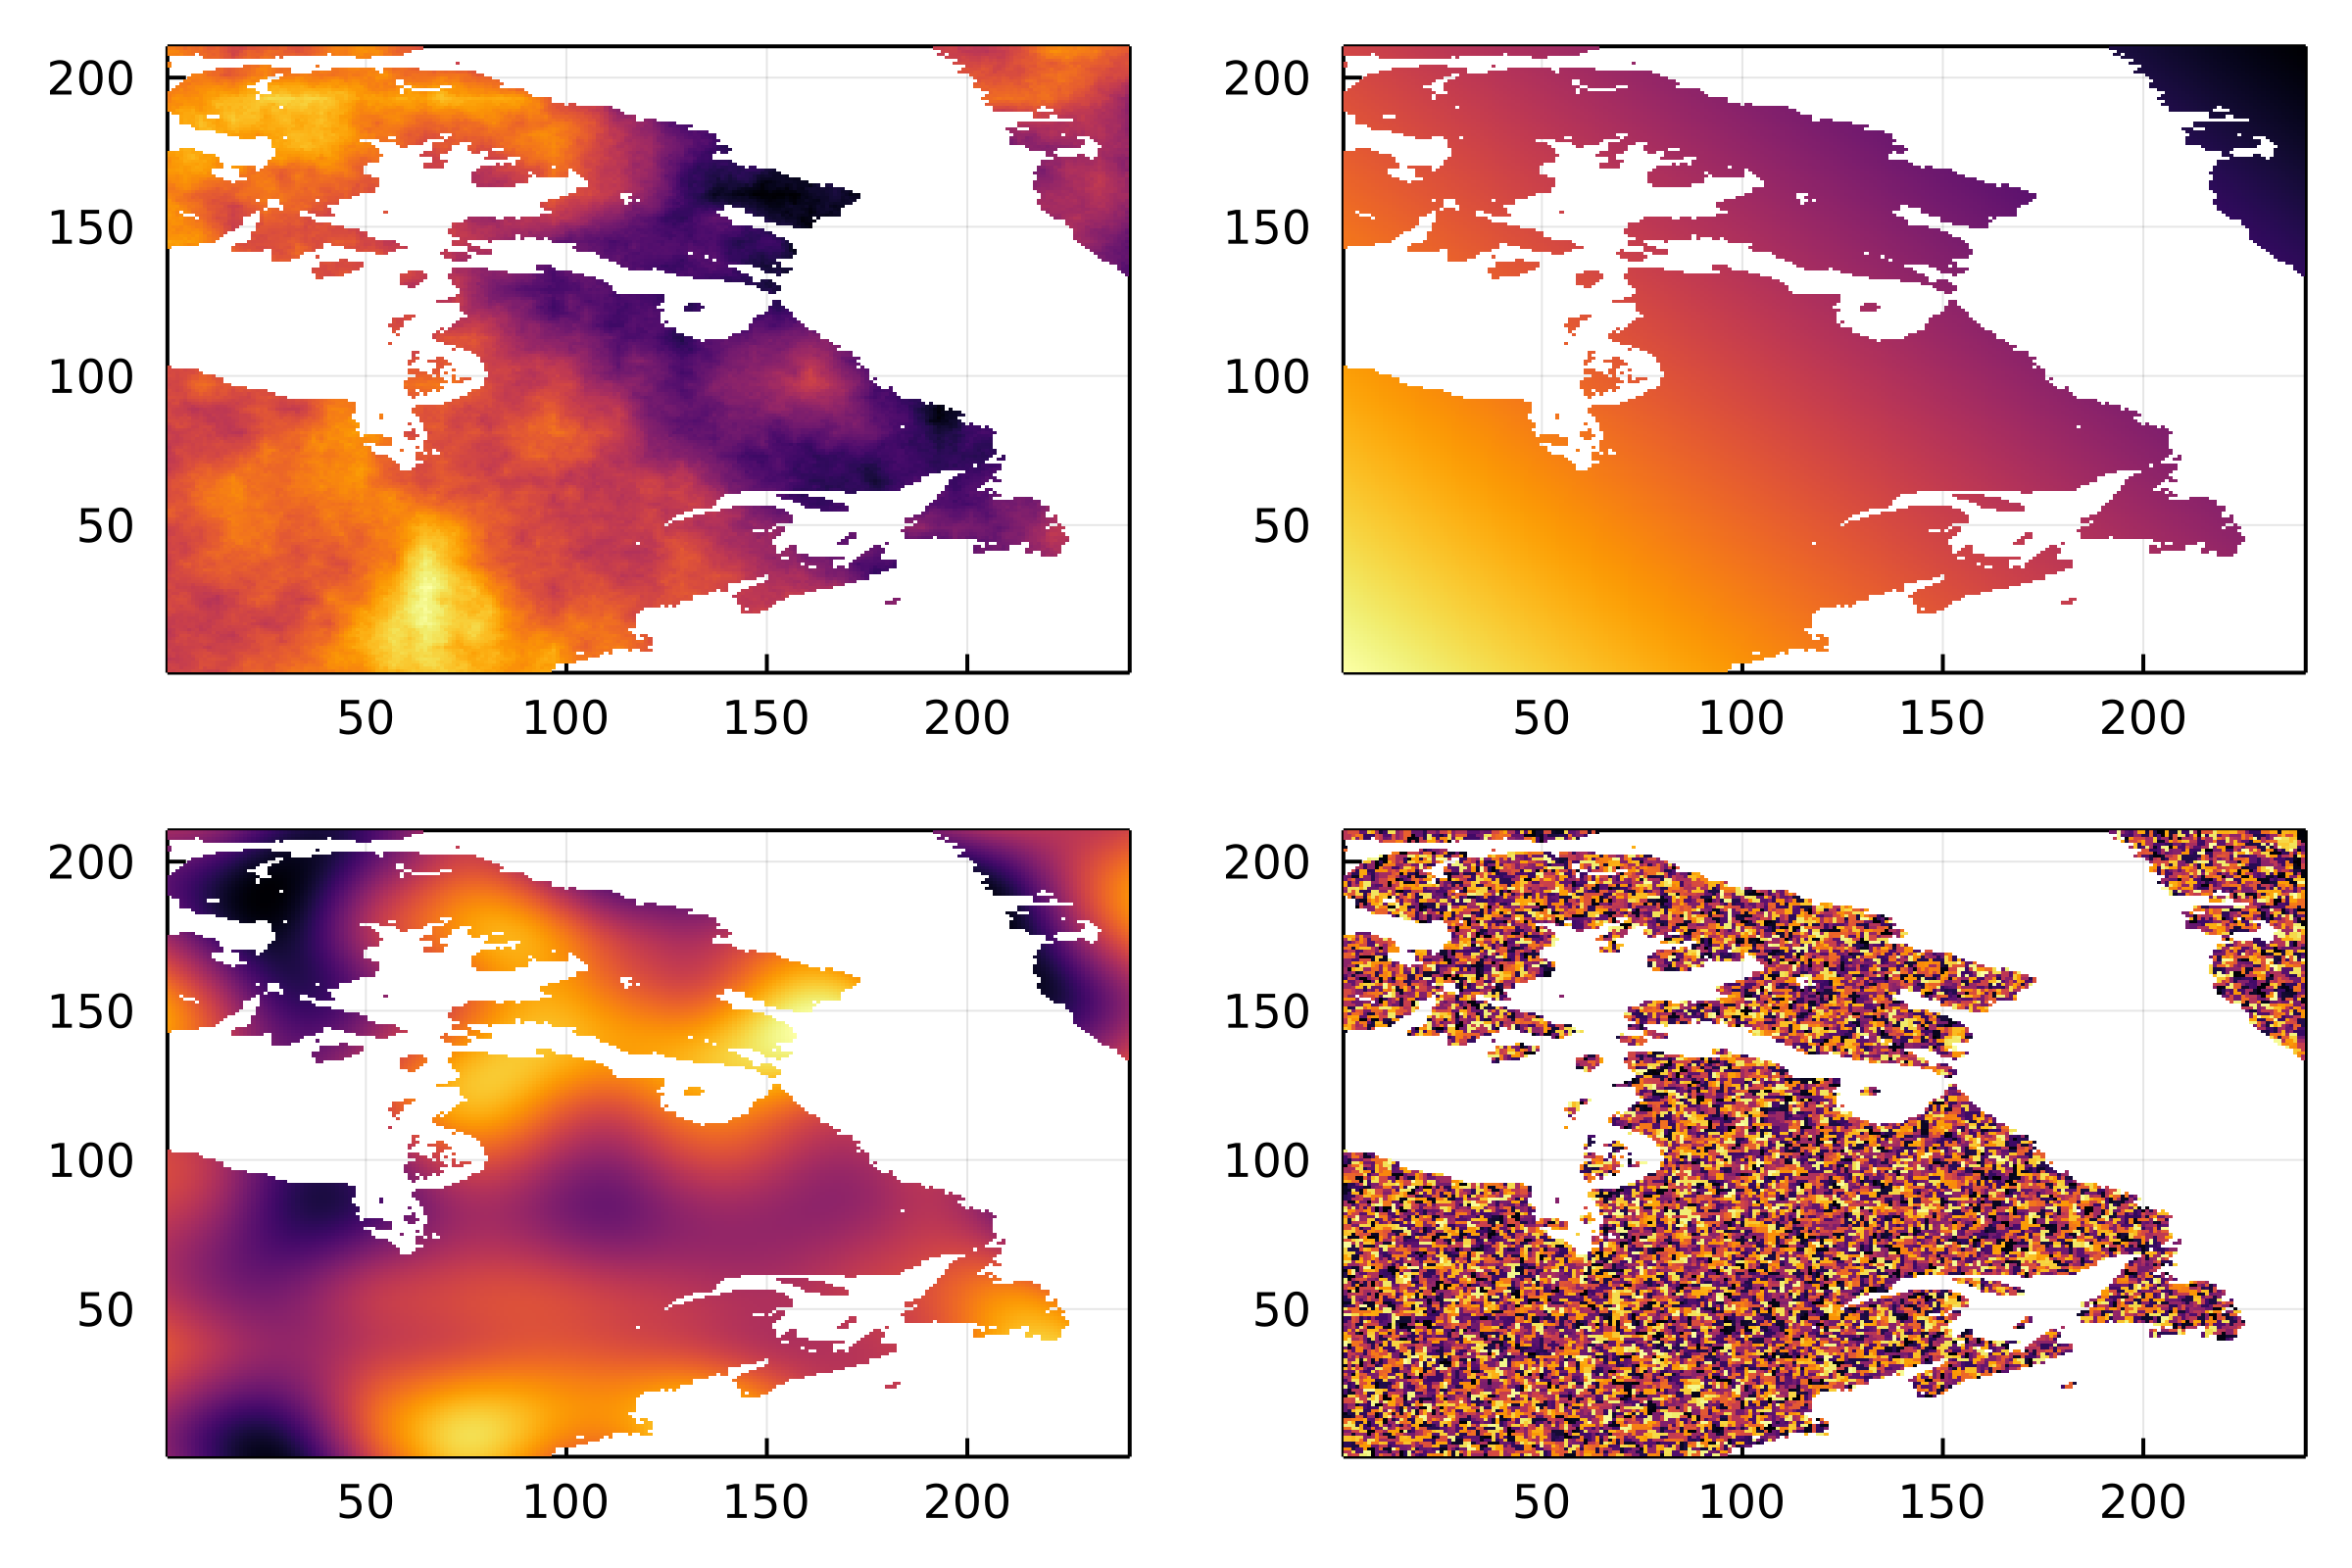
\includegraphics{./figures/interoperable.png}
\caption{todo}
\end{figure}

\hypertarget{rescaling-to-mimic-real-data}{%
\subsection{Rescaling to mimic real
data}\label{rescaling-to-mimic-real-data}}

Figure: Real temp (left) / Rescaled NL (right) , same unit bar

\hypertarget{generating-dynamic-neutral-landscapes}{%
\subsection{Generating dynamic neutral
landscapes}\label{generating-dynamic-neutral-landscapes}}

We implement methods for generating change that are temporally
autocorrelated, spatially-autocorrelated, or both.

\(M_t = M_{t-1} + f(M(t-1))\)

\hypertarget{models-of-change}{%
\subsection{Models of change}\label{models-of-change}}

Two types of temporal change: (1) null change, where the is random
variation in each cell across time but the mean value across all cells
stays constant (with some variation around this constant due to
randomness in change generation)

\hypertarget{null}{%
\subsubsection{Null}\label{null}}

Take an arbitrary distribution (from \texttt{Distributions.jl}) and set
its mean value to 0, and apply draws from that distribution to each cell
at each timestep.

\hypertarget{directional}{%
\subsubsection{Directional}\label{directional}}

Can take an arbitrary distribution of values and set its expected-value
to be the primary input into a change model---the mean amount of change
at each timestep. This can also be parameterized to a be a variable list
of mean change at each corresponding timestep.

\hypertarget{temporally-autocorrelation}{%
\paragraph{Temporally
autocorrelation}\label{temporally-autocorrelation}}

We generate temporally autocorrelated change using the method. We take
an arbitrary distribution \(A\)

\(r\): rate, \(v\): variability, \(U\) matrix of draws from standard
\(\text{Normal}(0,1)\). Here \(v\) replects the amount of temporal
autocorrelation.

The value of a given cell \((i,j)\) with value \(M_{ij}\)
\[M_{ij}(t+1) = f_{T}(M_{ij}(t)) = r + vA_{ij}\]

Results in an expected value of change of \(r\) per timestep with
variance \(v\).

\hypertarget{spatial-autocorrelation}{%
\paragraph{Spatial autocorrelation}\label{spatial-autocorrelation}}

Generate a matrix \(\delta\) with a NL generator.

\(r\): rate, \(v\): variability, \([Z(\delta)]_{ij}\): the \((i,j)\)
entry of the z-score of the \(\delta\) matrix

Z-score is arbitrary and can be replaced with any dist.

\(f_{S}(M_{ij}) = r + v \cdot [Z(\delta)]_{ij}\)

\hypertarget{spatiotemporal-autocorrelation}{%
\paragraph{Spatiotemporal
autocorrelation}\label{spatiotemporal-autocorrelation}}

Finally, to implement change this is both spatially and temporally
autocorrelated

\(f_{ST}(M_{ij}) = r + v \cdot [Z(\delta)]_{ij}\)

\begin{figure}
\centering
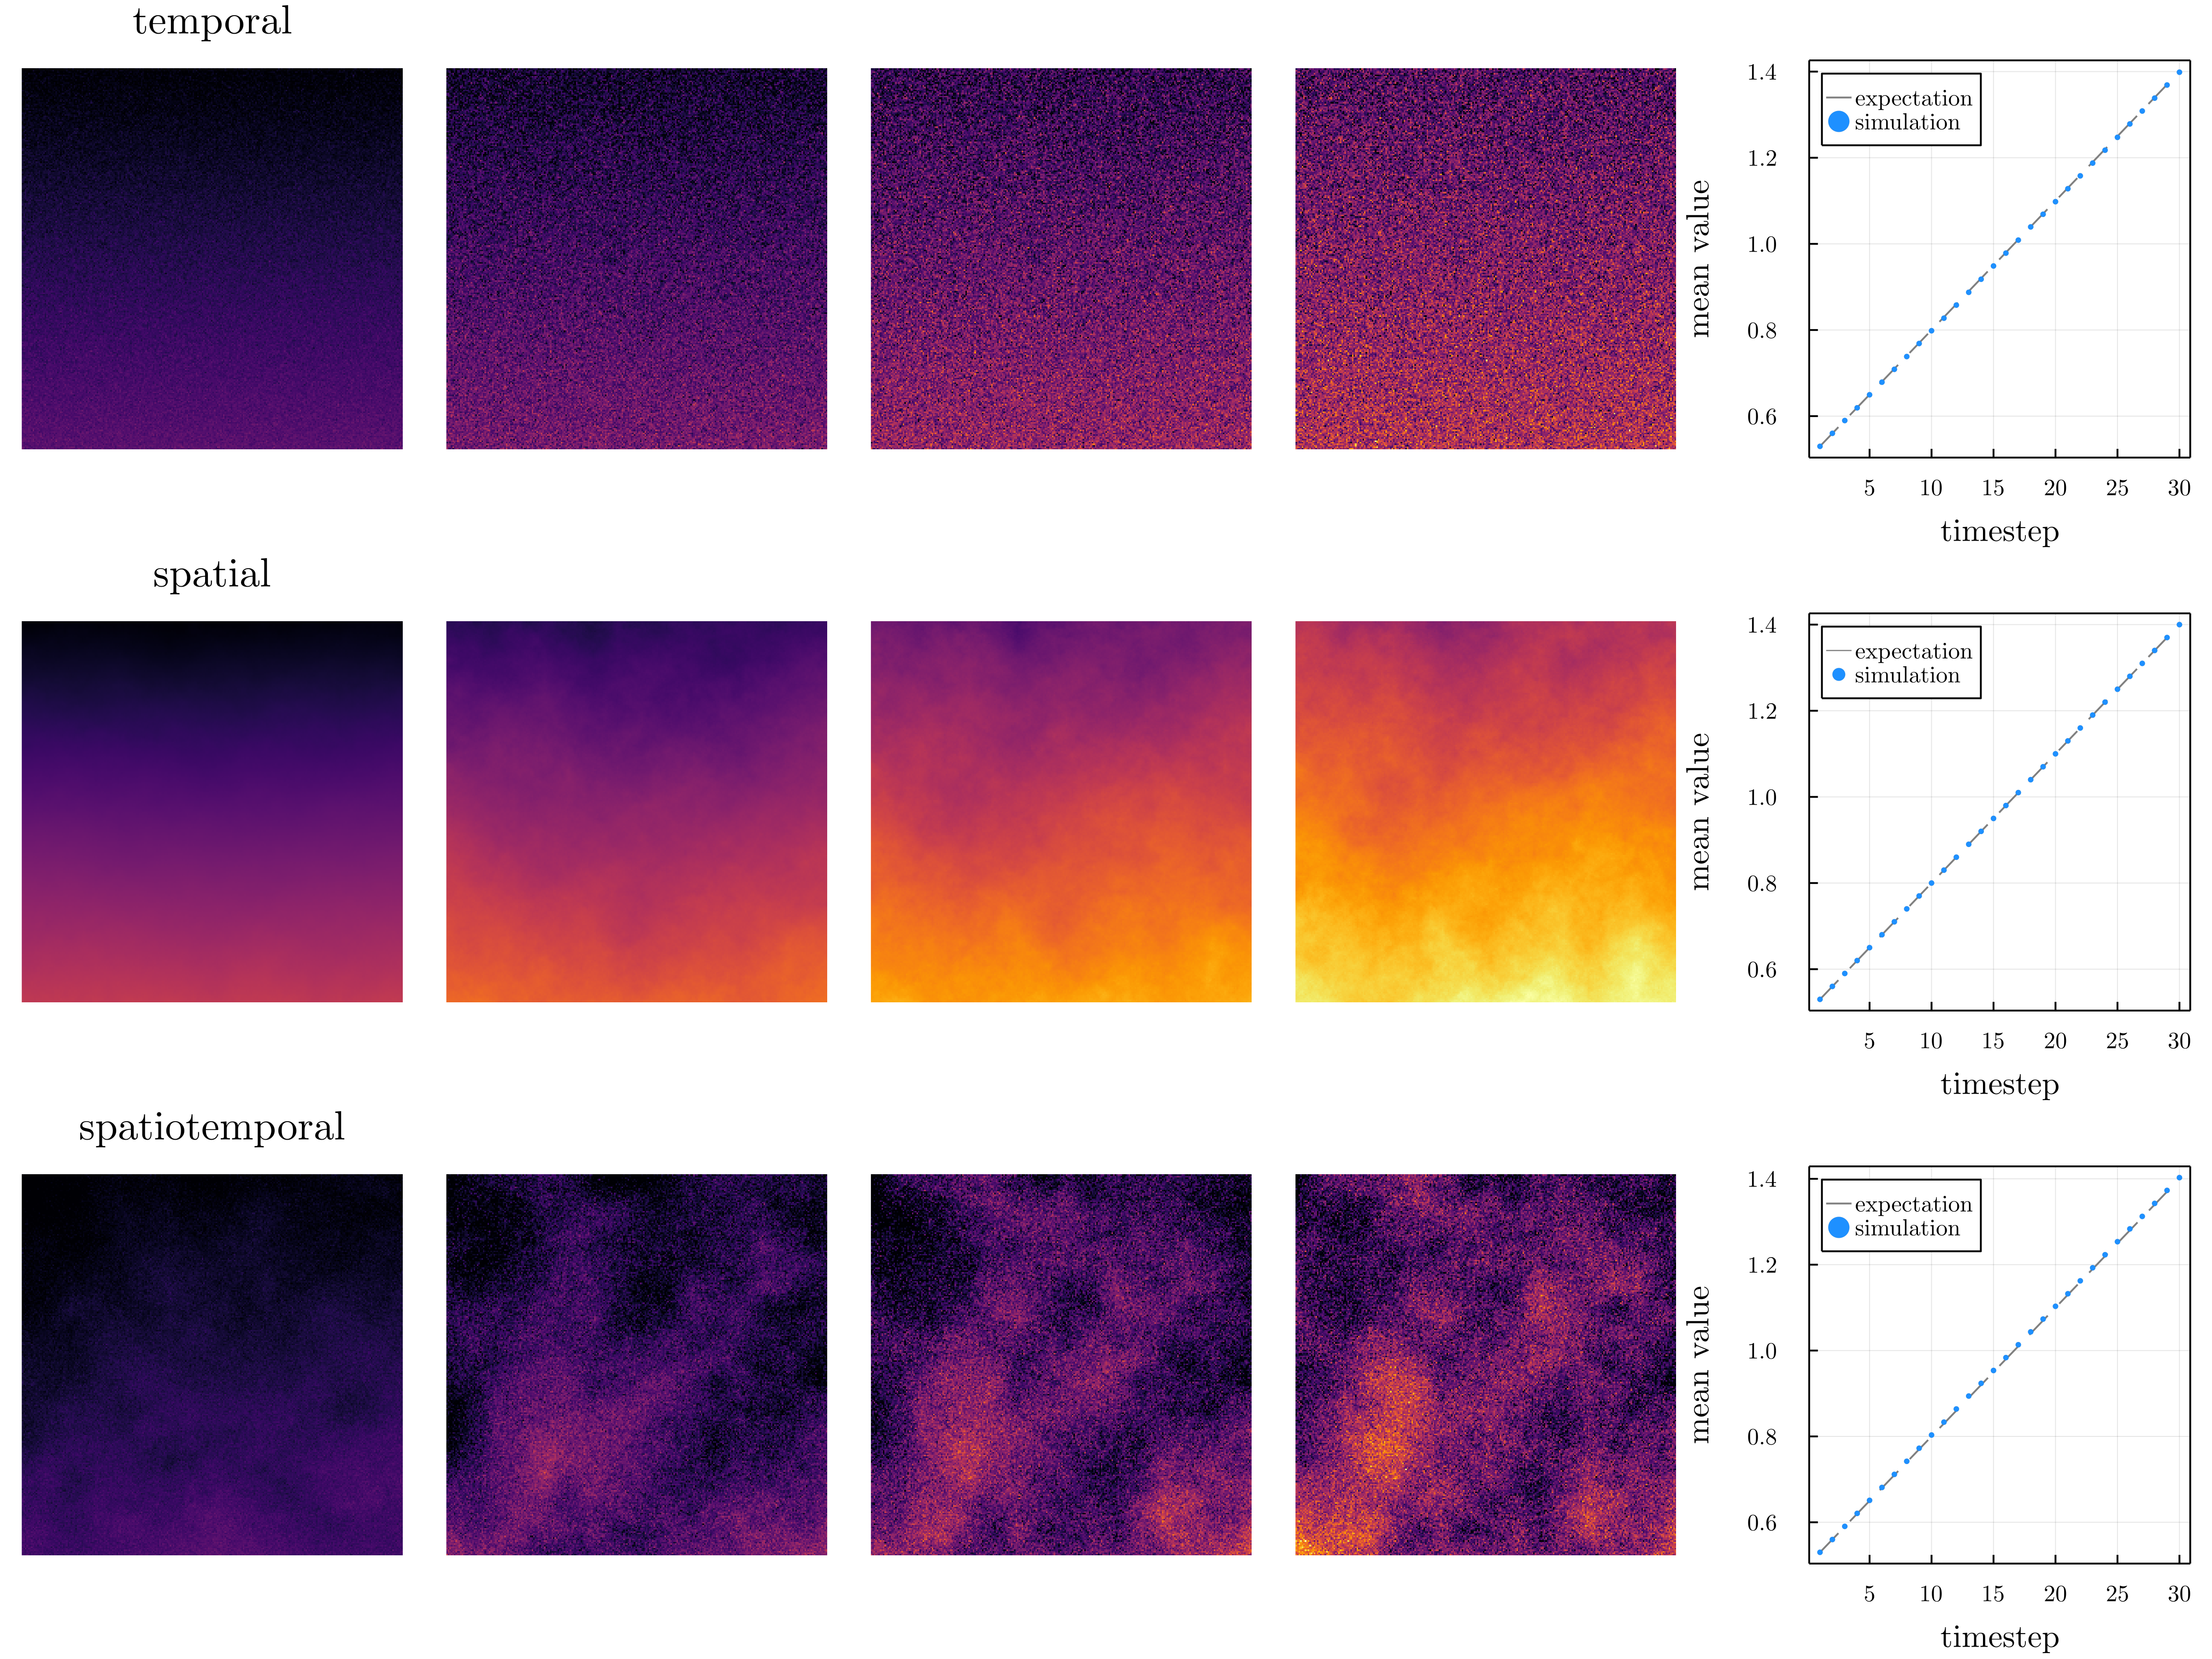
\includegraphics{./figures/temporal.png}
\caption{todo}
\end{figure}

\hypertarget{benchmark-comparison-to-nlmpy-and-nlmr}{%
\section{\texorpdfstring{Benchmark comparison to \texttt{nlmpy} and
\texttt{NLMR}}{Benchmark comparison to nlmpy and NLMR}}\label{benchmark-comparison-to-nlmpy-and-nlmr}}

It's fast. As the scale and resolution of raster data increases, neutral
models must be able to scale to match those data dimensions.

\begin{figure}
\centering
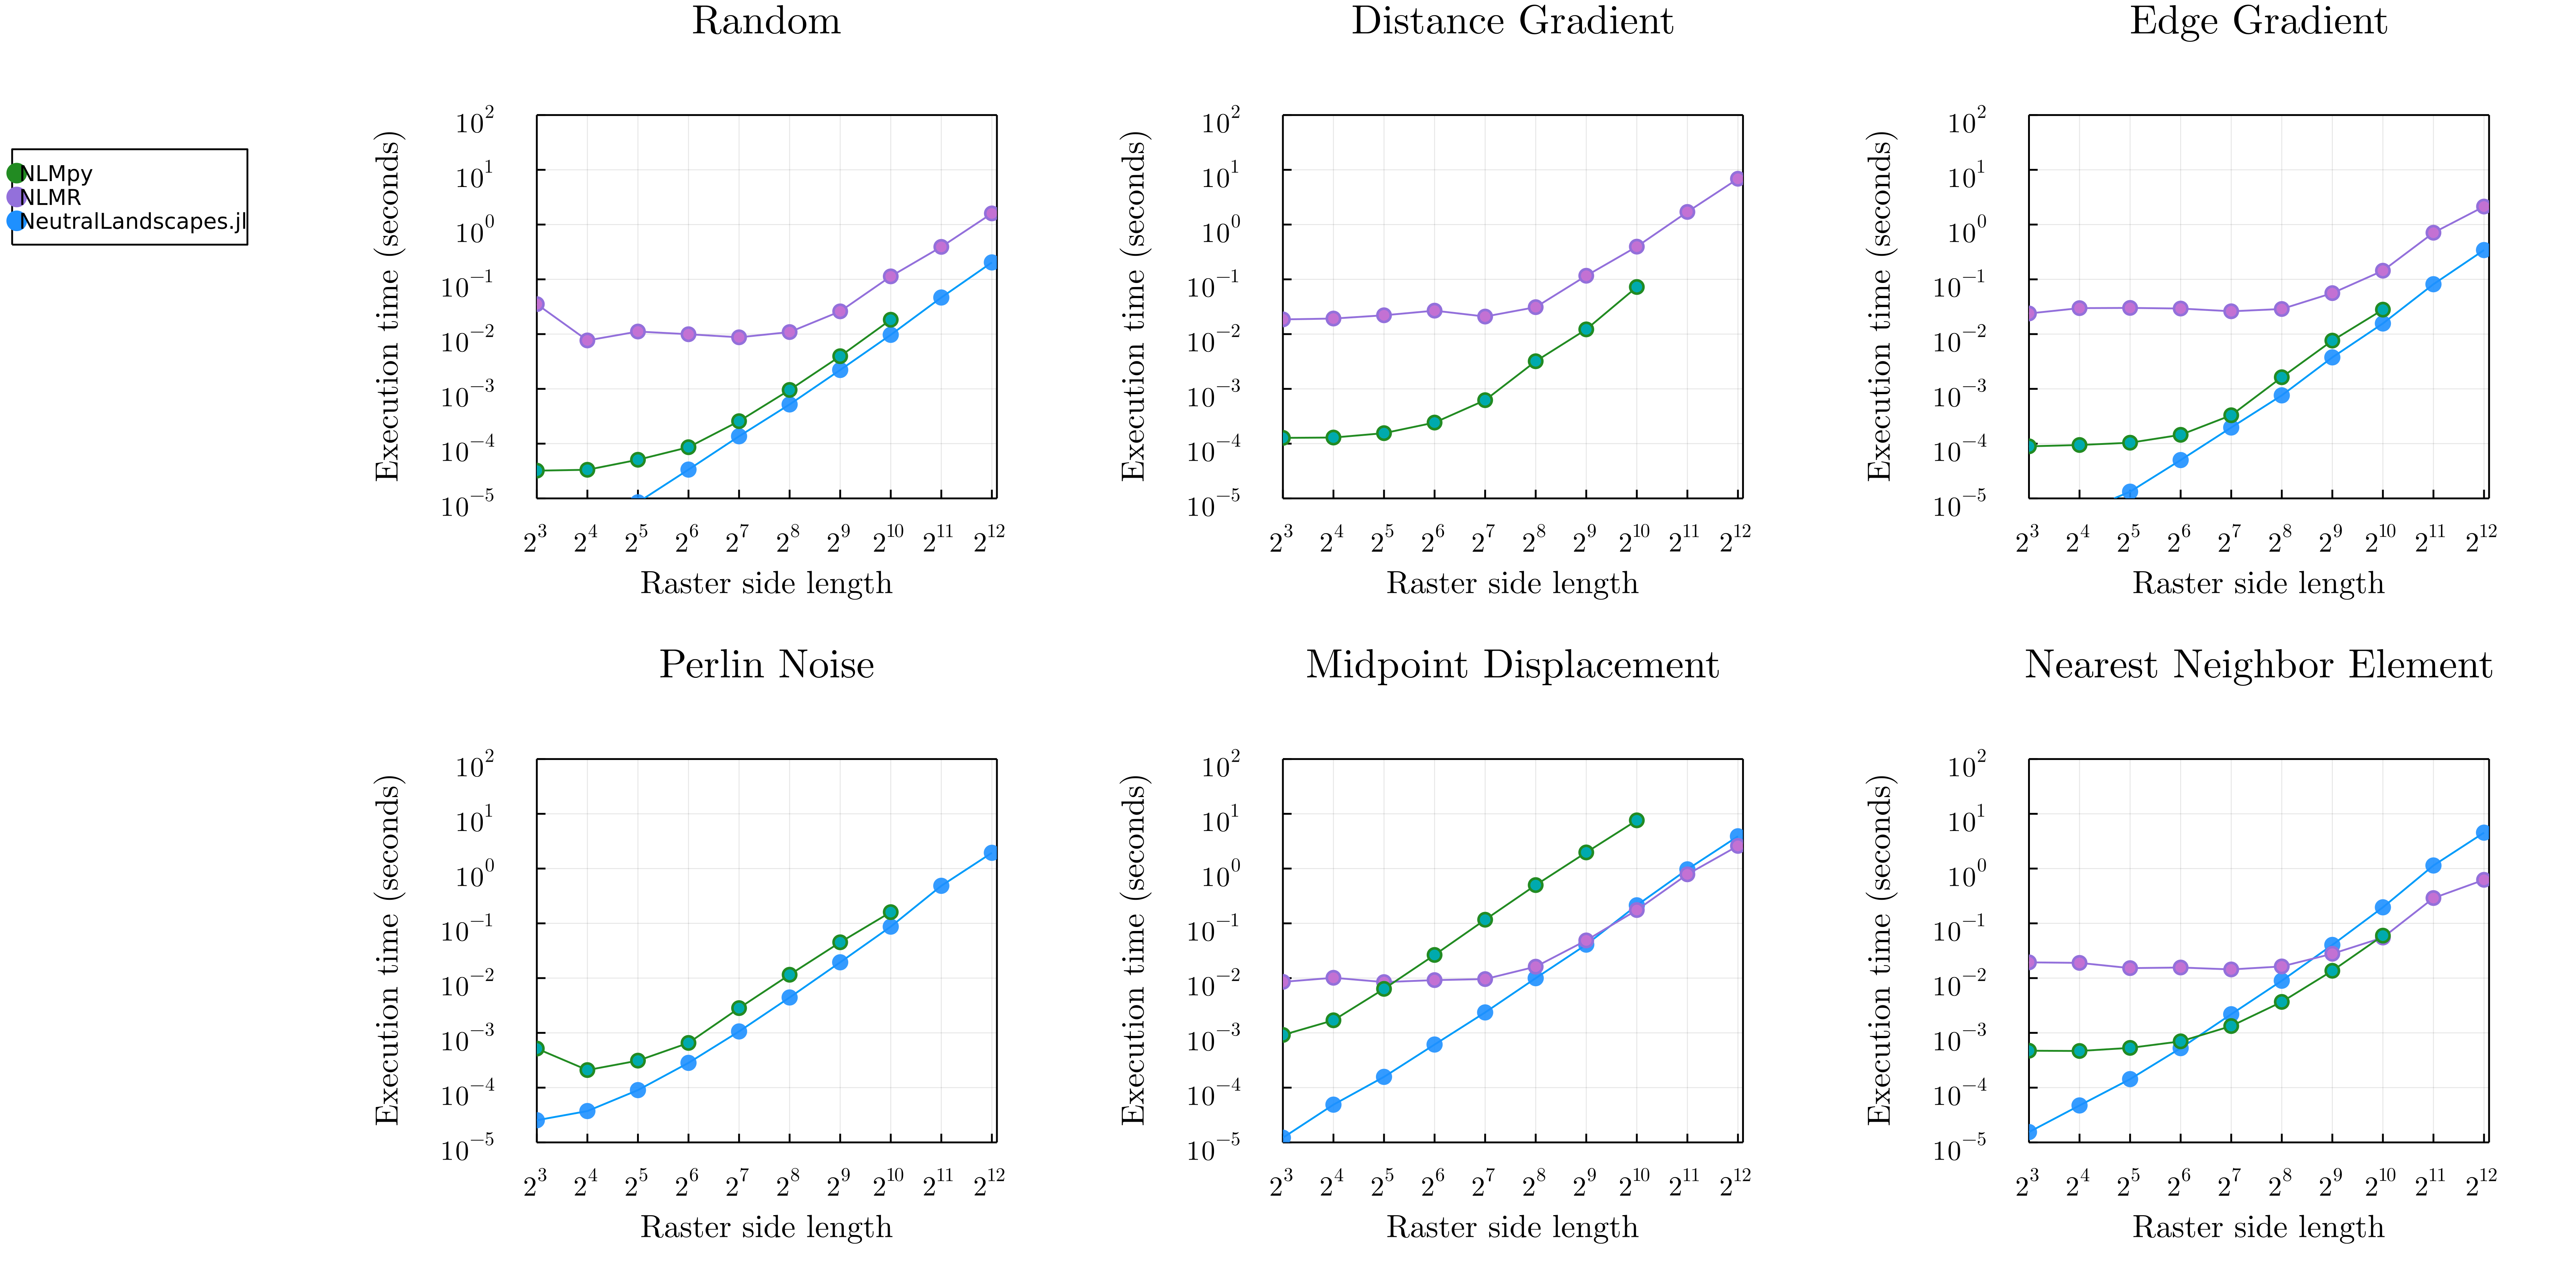
\includegraphics{./figures/benchmark.png}
\caption{todo}
\end{figure}

How many lines of code, and what language is that code in for each pkg?
\texttt{NLMR} contains 893 lines of R, and 376+51 lines of C++.
\texttt{nlmpy} contains 386 lines of python. Julia contains 664 lines of
(non-test) \texttt{julia}. Note these numbers refer only to lines of
code and not comments.

\hypertarget{example-fitting-a-neutral-landscape-to-an-empirical-spatial-dataset-using-generative-modeling}{%
\section{Example: fitting a neutral landscape to an empirical spatial
dataset using generative
modeling}\label{example-fitting-a-neutral-landscape-to-an-empirical-spatial-dataset-using-generative-modeling}}

Here we use approximate bayesian computation to estimate the parameter
of autocorrelation H for an empirical raster of temperature data.

Why? What if we are interested in differentiating the processes that
occur in this \emph{real} landscape versus landscapes with \emph{similar
statistical properties}.

We take a raster of mean temp around the st lawrence lowlands in QC, and
use ABC to estimate the value of H under the midpoint-displacement
model.

We use the variogram as the loss function

\begin{figure}
\hypertarget{fig:post}{%
\centering
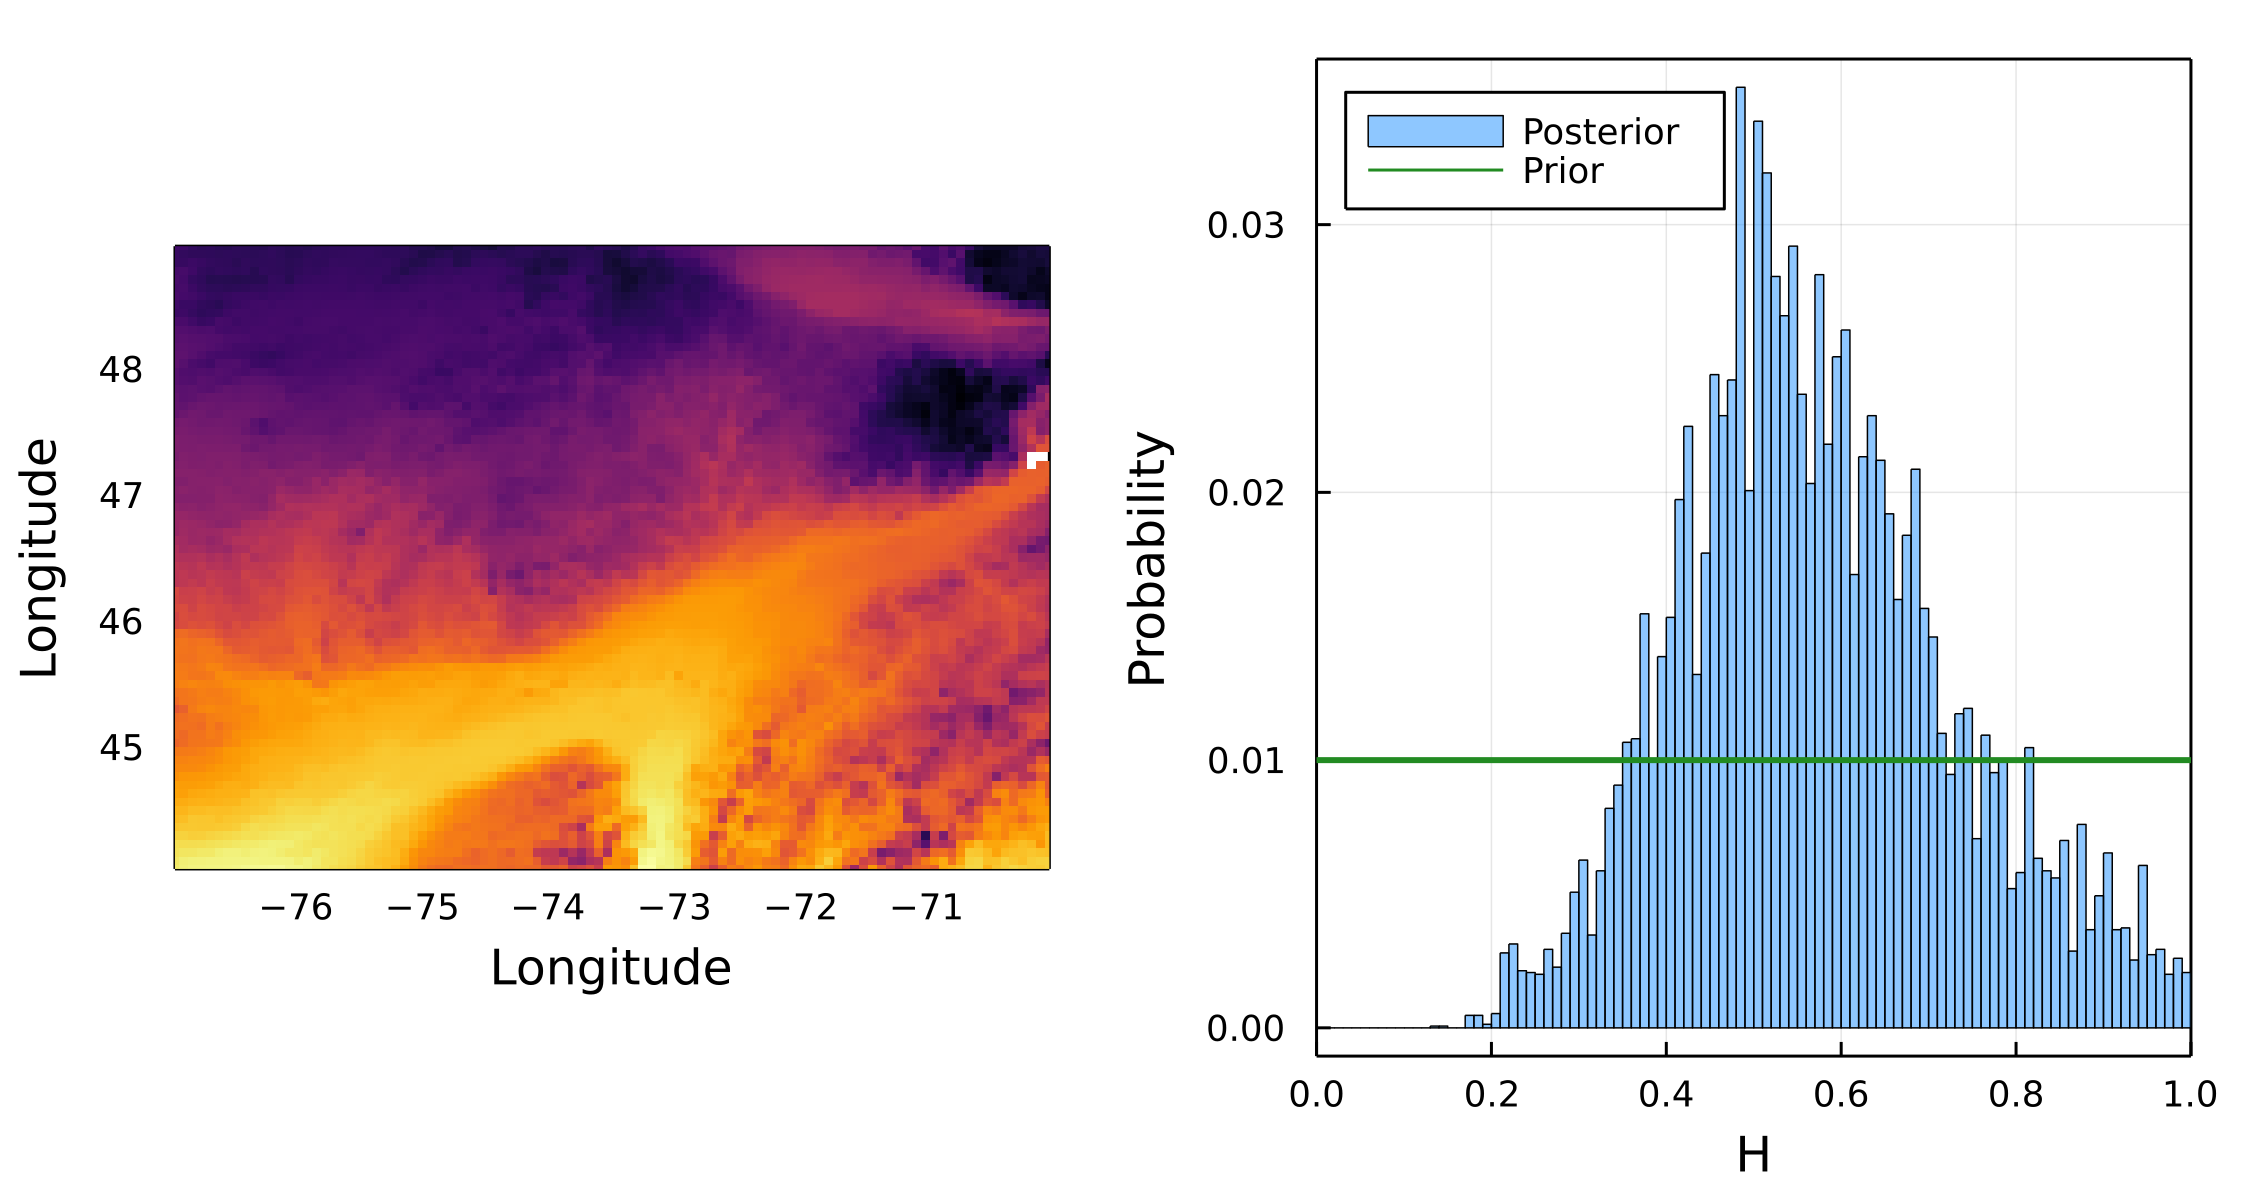
\includegraphics{./figures/posterior.png}
\caption{todo}\label{fig:post}
}
\end{figure}

\hypertarget{discussion}{%
\section{Discussion}\label{discussion}}

Why is it good that we've made this a faster thing to do? Why are models
of temporal change necessary? What can simulation do for spatial ecology
more generally?

What are questions we can address with NL.jl that was not possible
before?

\hypertarget{references}{%
\section*{References}\label{references}}
\addcontentsline{toc}{section}{References}

\hypertarget{refs}{}
\begin{CSLReferences}{1}{0}
\leavevmode\hypertarget{ref-Albert2017BarDis}{}%
Albert, J.S., Schoolmaster, D.R., JR., Tagliacollo, V. \&
Duke-Sylvester, S.M. (2017). Barrier Displacement on a Neutral
Landscape: Toward a Theory of Continental Biogeography. \emph{Systematic
Biology}, 66, 167--182.

\leavevmode\hypertarget{ref-Etherington2015NlmPyt}{}%
Etherington, T.R., Holland, E.P. \& O'Sullivan, D. (2015). NLMpy: A
python software package for the creation of neutral landscape models
within a general numerical framework. \emph{Methods in Ecology and
Evolution}, 6, 164--168.

\leavevmode\hypertarget{ref-Gardner1987NeuMod}{}%
Gardner, R.H., Milne, B.T., Turnei, M.G. \& O'Neill, R.V. (1987).
Neutral models for the analysis of broad-scale landscape pattern.
\emph{Landscape Ecology}, 1, 19--28.

\leavevmode\hypertarget{ref-Milne1992SpaAgg}{}%
Milne, B.T. (1992). Spatial Aggregation and Neutral Models in Fractal
Landscapes. \emph{The American Naturalist}, 139, 32--57.

\leavevmode\hypertarget{ref-Remmel2013CatCla}{}%
Remmel, T.K. \& Fortin, M.-J. (2013). Categorical, class-focused map
patterns: Characterization and comparison. \emph{Landscape Ecology}, 28,
1587--1599.

\leavevmode\hypertarget{ref-Sciaini2018NlmLan}{}%
Sciaini, M., Fritsch, M., Scherer, C. \& Simpkins, C.E. (2018). NLMR and
landscapetools: An integrated environment for simulating and modifying
neutral landscape models in R. \emph{Methods in Ecology and Evolution},
9, 2240--2248.

\leavevmode\hypertarget{ref-Storfer2007PutLan}{}%
Storfer, A., Murphy, M.A., Evans, J.S., Goldberg, C.S., Robinson, S.,
Spear, S.F., \emph{et al.} (2007). Putting the {``landscape''} in
landscape genetics. \emph{Heredity}, 98, 128--142.

\leavevmode\hypertarget{ref-Tinker2004HisRan}{}%
Tinker, D., Romme, W.H. \& Despain, D. (2004). Historic range of
variability in landscape structure in subalpine forests of the Greater
Yellowstone Area, USA. \emph{Landscape Ecology}.

\end{CSLReferences}

\end{document}
